\section{Effects of the PMT Saturation on the Position Reconstruction}
\label{secPosRecSaturation}

\begin{figure}[!h]
\centering
\subfigure[$^{137}$Cs]{
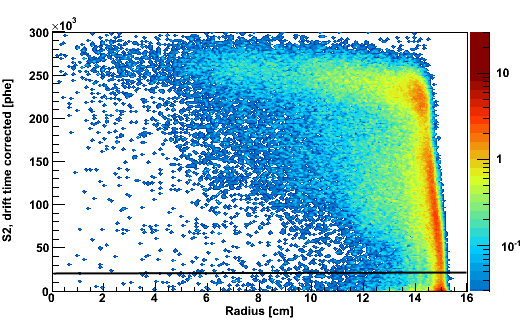
\includegraphics[width=0.475\linewidth]{plots/Saturation/S2vsR_Cs137_nn1_withLine.png}
\label{figS2vsR_1}}
\subfigure[$^{241}$Am-Be]{
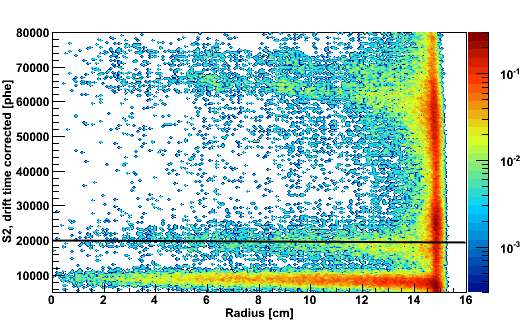
\includegraphics[width=0.475\linewidth]{plots/Saturation/S2vsR_AmBe_nn1_withLine.png}
\label{figS2vsR_2}}
\caption[S2 as a function of the TPC radius for the $^{137}$Cs calibration data, and for the $\gamma$-lines in the data acquired with $^{241}$Am-Be source]{S2 as a function of the TPC radius for the $^{137}$Cs calibration data (a), and for the lines in the data acquired with $^{241}$Am-Be source (b), induced by inelastic neutron scatters on xenon isotopes. The black lines indicate the region where PMT non-linearity effects take place. The reconstructed radii of the events close to the edge of the target volume are biased inwards above this lines.}
\label{figS2vsR}
\end{figure}

\begin{figure}[!h]
\centering
\subfigure[40~keV]{
%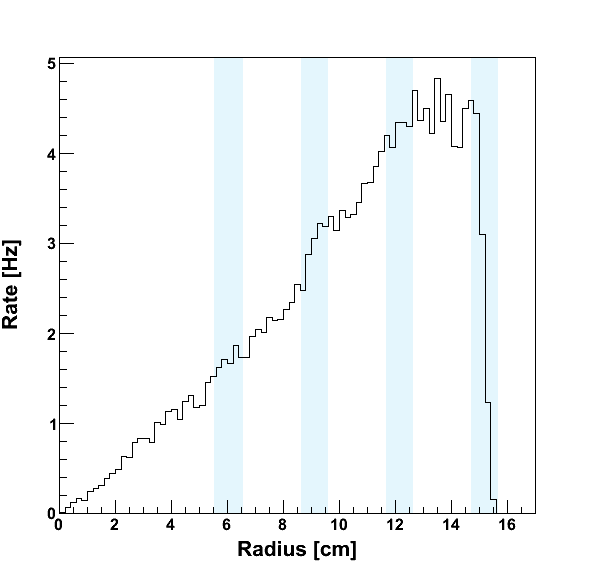
\includegraphics[height=0.4\linewidth]{plots/Saturation/c_r1_nn1_85bins_Saturation-L1-withLines1.png}
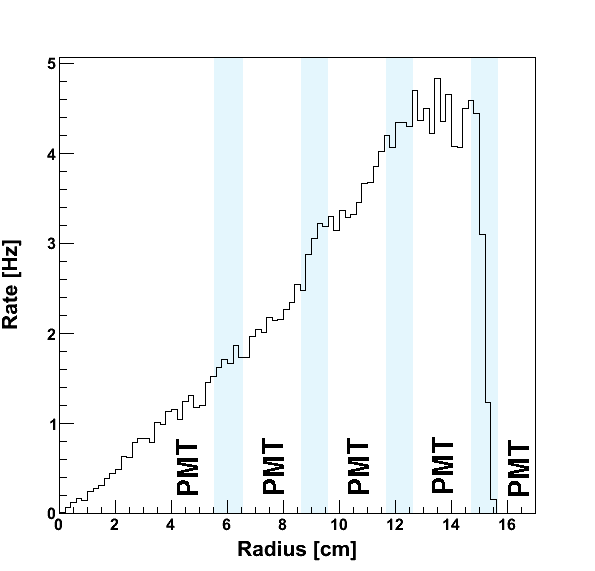
\includegraphics[height=0.35\linewidth]{plots/Saturation/c_r1_nn1_85bins_Saturation-L1-withLinesAndLabels.png}
\label{figRdeviation_1}}
\subfigure[80~keV]{
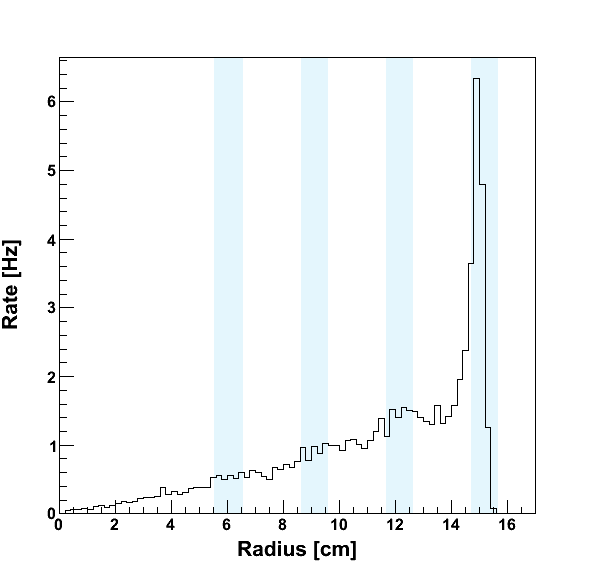
\includegraphics[height=0.35\linewidth]{plots/Saturation/c_r1_nn1_85bins_Saturation-L2-withLines1.png}
\label{figRdeviation_2}}
\subfigure[164~keV]{
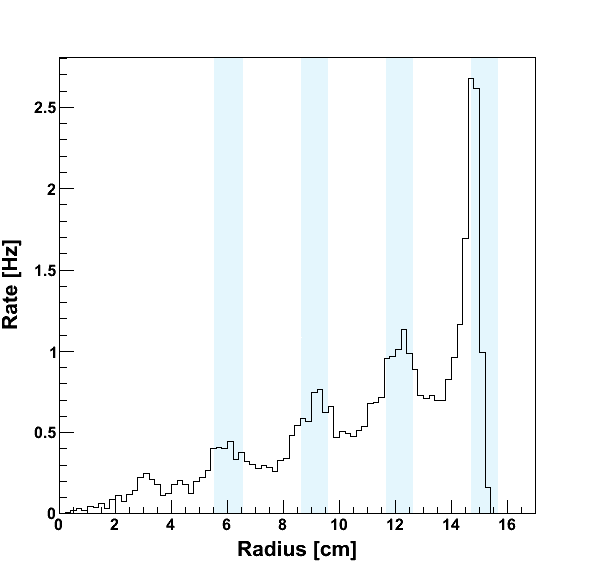
\includegraphics[height=0.35\linewidth]{plots/Saturation/c_r1_nn1_85bins_Saturation-L3-withLines1.png}
\label{figRdeviation_3}}
\subfigure[236~keV]{
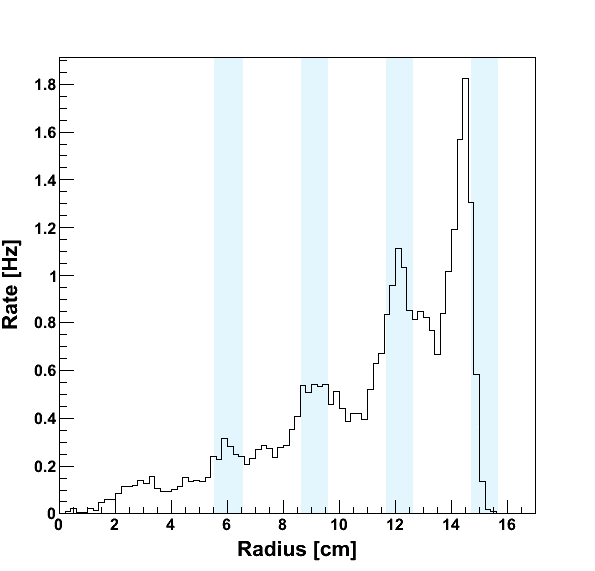
\includegraphics[height=0.35\linewidth]{plots/Saturation/c_r1_nn1_85bins_Saturation-L4-withLines1.png}
\label{figRdeviation_4}}
\caption[Deviation of the reconstructed radii for gammas of different energy]{Deviation of the reconstructed radii for gammas of different energy: (a) - 40~keV from inelastic neutron scatters on $^{129}$Xe; (b) - 80~keV from inelastic neutron scatters on $^{131}$Xe; (c) - 164~keV from de-excitation of $^{131\mathrm{m}}$Xe; (d) - 236~keV from de-excitation of $^{129\mathrm{m}}$Xe. The blue shaded lines show the position of the rows of PMTs within the top array.}
\label{figRdeviation}
\end{figure}

For light signals of high amplitude, the output current of a given PMT is no longer proportional to the incident light intensity, which is called saturation effect. The correlation between the size of the S2 signal and reconstructed radial positions is shown in Fig.~\ref{figS2vsR_1} and Fig.~\ref{figS2vsR_2}, for the $^{137}$Cs and $^{241}$Am-Be calibration data, respectively. The deviation of the reconstructed radius starts for S2 signals above $\sim$20'000  PE, which corresponds to an energy of electronic recoils of $\sim$80~keV.

The radial distributions of electronic recoils from the lines of different energies, induced by inelastic interactions of neutrons from an $^{241}$Am-Be source, are shown in Fig.~\ref{figRdeviation}. The regions between the concentric PMT rings in the top array are indicated by  the light blue background. Two effects in the imperfect position reconstruction can be seen, both resulting from the PMT saturation. 
First, when the size of the S2 signal increases, the reconstructed radii of the events close to the edge of the target volume are biased inwards, towards the inner PMT ring. Second, for S2 light saturating the phototubes, the output signals of the PMTs from different radii have a similar size. Therefore, a fake minimum is found by the position reconstruction algorithm, and the events are reconstructed between the PMT rings.

Due to this problem, some of the calibrations, such as with $^{137}$Cs to infer the position dependent light yield map in the TPC, have been performed with the lower anode voltage (2.2 to 3.0~kV), leading to a much smaller S2 signal which is less affected by PMT saturation.




%\begin{figure}[!h]
%\centering
%\subfigure[]{
%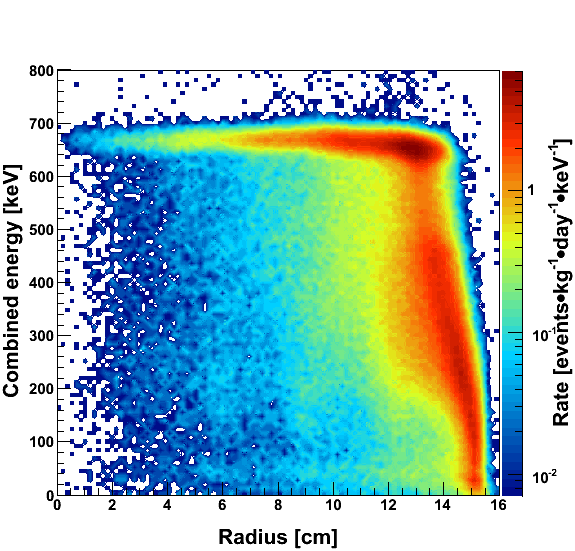
\includegraphics[width=0.475\linewidth]{plots/Saturation/CEvsR_Cs.png}
%\label{figCEvsR_1}}
%\subfigure[]{
%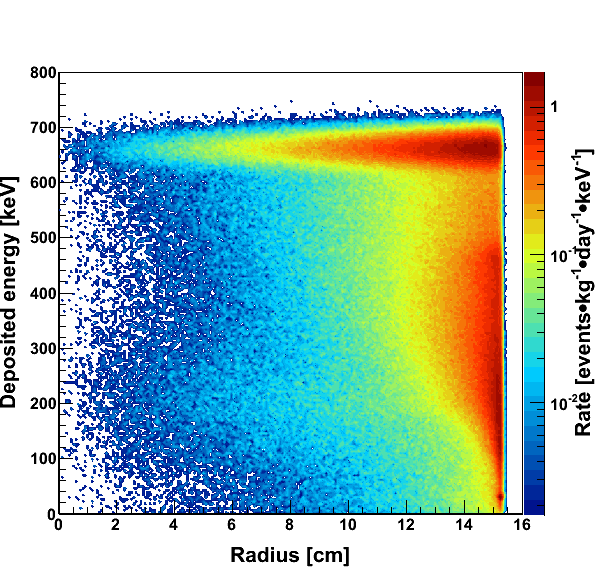
\includegraphics[width=0.475\linewidth]{plots/Saturation/EvsR_MC_Cs137.png}
%\label{figCEvsR_2}}
%\caption{Reconstructed energy as a function of the TPC radius for $^{137}$Cs calibration data. Monte Carlo simulation.}
%\label{figCEvsR}
%\end{figure}
